\chapter{Luminosity  Measurement and Calibration}
\label{ch3}

Accurately measuring the luminosity delivered to the CMS experiment by the LHC is essential for various reasons. Online, the luminosity measurement provides feedback on the LHC and CMS performance and operations, including measuring trigger rates. In offline analysis, the luminosity measurement is a critical component for measuring the cross-section of observed processes or setting upper limits in searches for processes beyond the standard model.

As we see, to measure luminosity, a total of seven luminometers are used at CMS, and each of them reads out a specific quantity observed in the detector, such as hits, tracks, or clusters. The rate R measured by the luminometer is proportional to the instantaneous luminosity, $\mathcal{L}_{inst}$, with the constant of proportionality given by the visible cross-section $\sigma_{vis}$ \cite{pas_18}.

\begin{equation}
R(t)=\mathcal{L}_{inst}\sigma_{vis}
\label{lumi_exp_gen}
\end{equation}

The determination of $\sigma_{vis}$ is performed through van der Meer (vdM) scans using a specialized LHC machine setup. This chapter provides a description of this procedure, specifically applied with the PCC method.

\section{Pixel Cluster Counting method}

The PCC method utilizes the mean number of pixel clusters in the CMS silicon pixel detector to determine an offline luminosity measurement, this method exploits the very large number of pixels in the inner part of the CMS tracking system, it means that the probability of a given pixel being hit by two different charged particles from the same bunch crossing is exceedingly small, this large granularity and low occupancy yield measurements with excellent linear response with the pile-up (number of interactions per bunch crossing)$\mu$ \cite{PCC_PAS_12_001},  on average, the detector occupancy is less than 0.1\%\cite{lumi_precise_2015_2016}.\\ 

Figure \ref{pileup} shows a simulation with pp collision zero-bias events with the pixel cluster counting rate as a function of pileup in the pileup range observed in Run 2 from 0 to about 50 $\mu$. Where the mean number of pixel clusters is of the order of  111 per event. The red curve is a first-order polynomial fit with slope, a good agreement is seen based on the estimated goodness-of-fit $\chi^{2}$ per degree of freedom (dof) with a value of about 0.5, showing that the PCC rate is highly linear in this range under simulated conditions \cite{ Phase2_Upgrade,lumi_precise_2015_2016}.

\begin{center}
  \begin{figure}[h!]
    \centering
    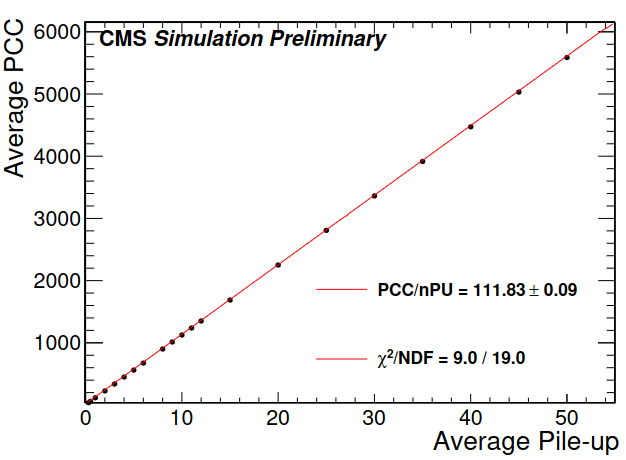
\includegraphics[scale=.35]{Chapter3/pileup_lineality.png} 
    \caption[Linearity with pile-up]{ Linearity of pixel cluster counting over the pileup range observed in Run 2 (from 0 to about 50) from simulation. The red line is a linear fit to the points \cite{Phase2_Upgrade} }
    \label{pileup}
  \end{figure}
\end{center}

To obtain the mean number of pixel clusters per event, several zero-bias events are averaged. This value is given by :

\begin{equation}
\left < N_{\text{cluster}} \right > \equiv \left < N_{\text{cluster}/\text{interaction}} \right > \mu
\end{equation}

Under minimum bias conditions, $\mu$ can be expressed as: 

\begin{equation}
\mu = \frac{\sigma_{\text{minBias}}}{f} \cdot \mathcal{L}_{inst}
\end{equation}

where $f$ is the LHC revolution frequency and $\mathcal{L}_{inst}$ is the single bunch instantaneous luminosity (SBIL). The minimum bias cross section $\sigma_{\text{minBias}}$ here is related to the PCC visible cross section by the mean number of clusters per interaction:

\begin{equation}
\sigma_{vis}= \left < N_{\text{cluster}/\text{interaction}} \right >\cdot \sigma_{\text{minBias}}
\end{equation}

Combining everything, the PCC luminosity measurement is obtained as:

\begin{equation}
\mathcal{L}_{inst}=\frac{\left < N_{\text{cluster}} \right >}{\sigma_{vis}} \cdot f
\end{equation}

%This method is capable of providing a precise luminosity measurement over longer time periods, but it cannot do so for a single luminosity section (23 seconds) as is possible with online luminometers. The reason for this limitation is the limited CMS trigger bandwidth available for collecting data \cite{pas_18}. A detailed discussion on this topic can be found in the next chapter.\\

%PCC si calcula lumi por cada lumi section.  Esto no tiene que ver con online vs offline.  PCC es un offline luminometro, quiere decir que los datos llegan tarde.  Con PCC solo podemos calcular lumi cada lumi section, debido a la baja estadistica (por la lectura de los datos de zero bias).  otros luminometros tienen precision con NB4 (HF, PLT, BCM1F).  

In the PCC measurement, the innermost layer of the pixel detector is excluded from the analysis due to significant dynamic inefficiency effects \cite{pas_18}. At higher $\mathcal{L}_{inst}$, the hit efficiency in this layer decreases because the readout chip cannot process all of the hits.\\ 

\section{2022 CMS Data collected}

On July 12th, 2022, the data collection for Run3 of the Large Hadron Collider (LHC) began, which resulted in a total recorded luminosity of $38.48 fb^{-1}$. This collection period encompassed the duration from the start of stable beams until the beam was dumped, or when stable beams ceased for other reasons, such as beam studies. The luminosity delivered by the LHC to CMS (blue) and the luminosity recorded by CMS (orange) during stable beams and proton-proton collisions at a center-of-mass energy of $\sqrt{s}$ 13.6 TeV in 2022 are depicted in Figure \ref{Lumi_2022}. Note that  the special runs that occurred at injection energy (450 GeV) are not represented in these graphs \citep{wikicern}.

\begin{center}
  \begin{figure}[h!]
    \centering
    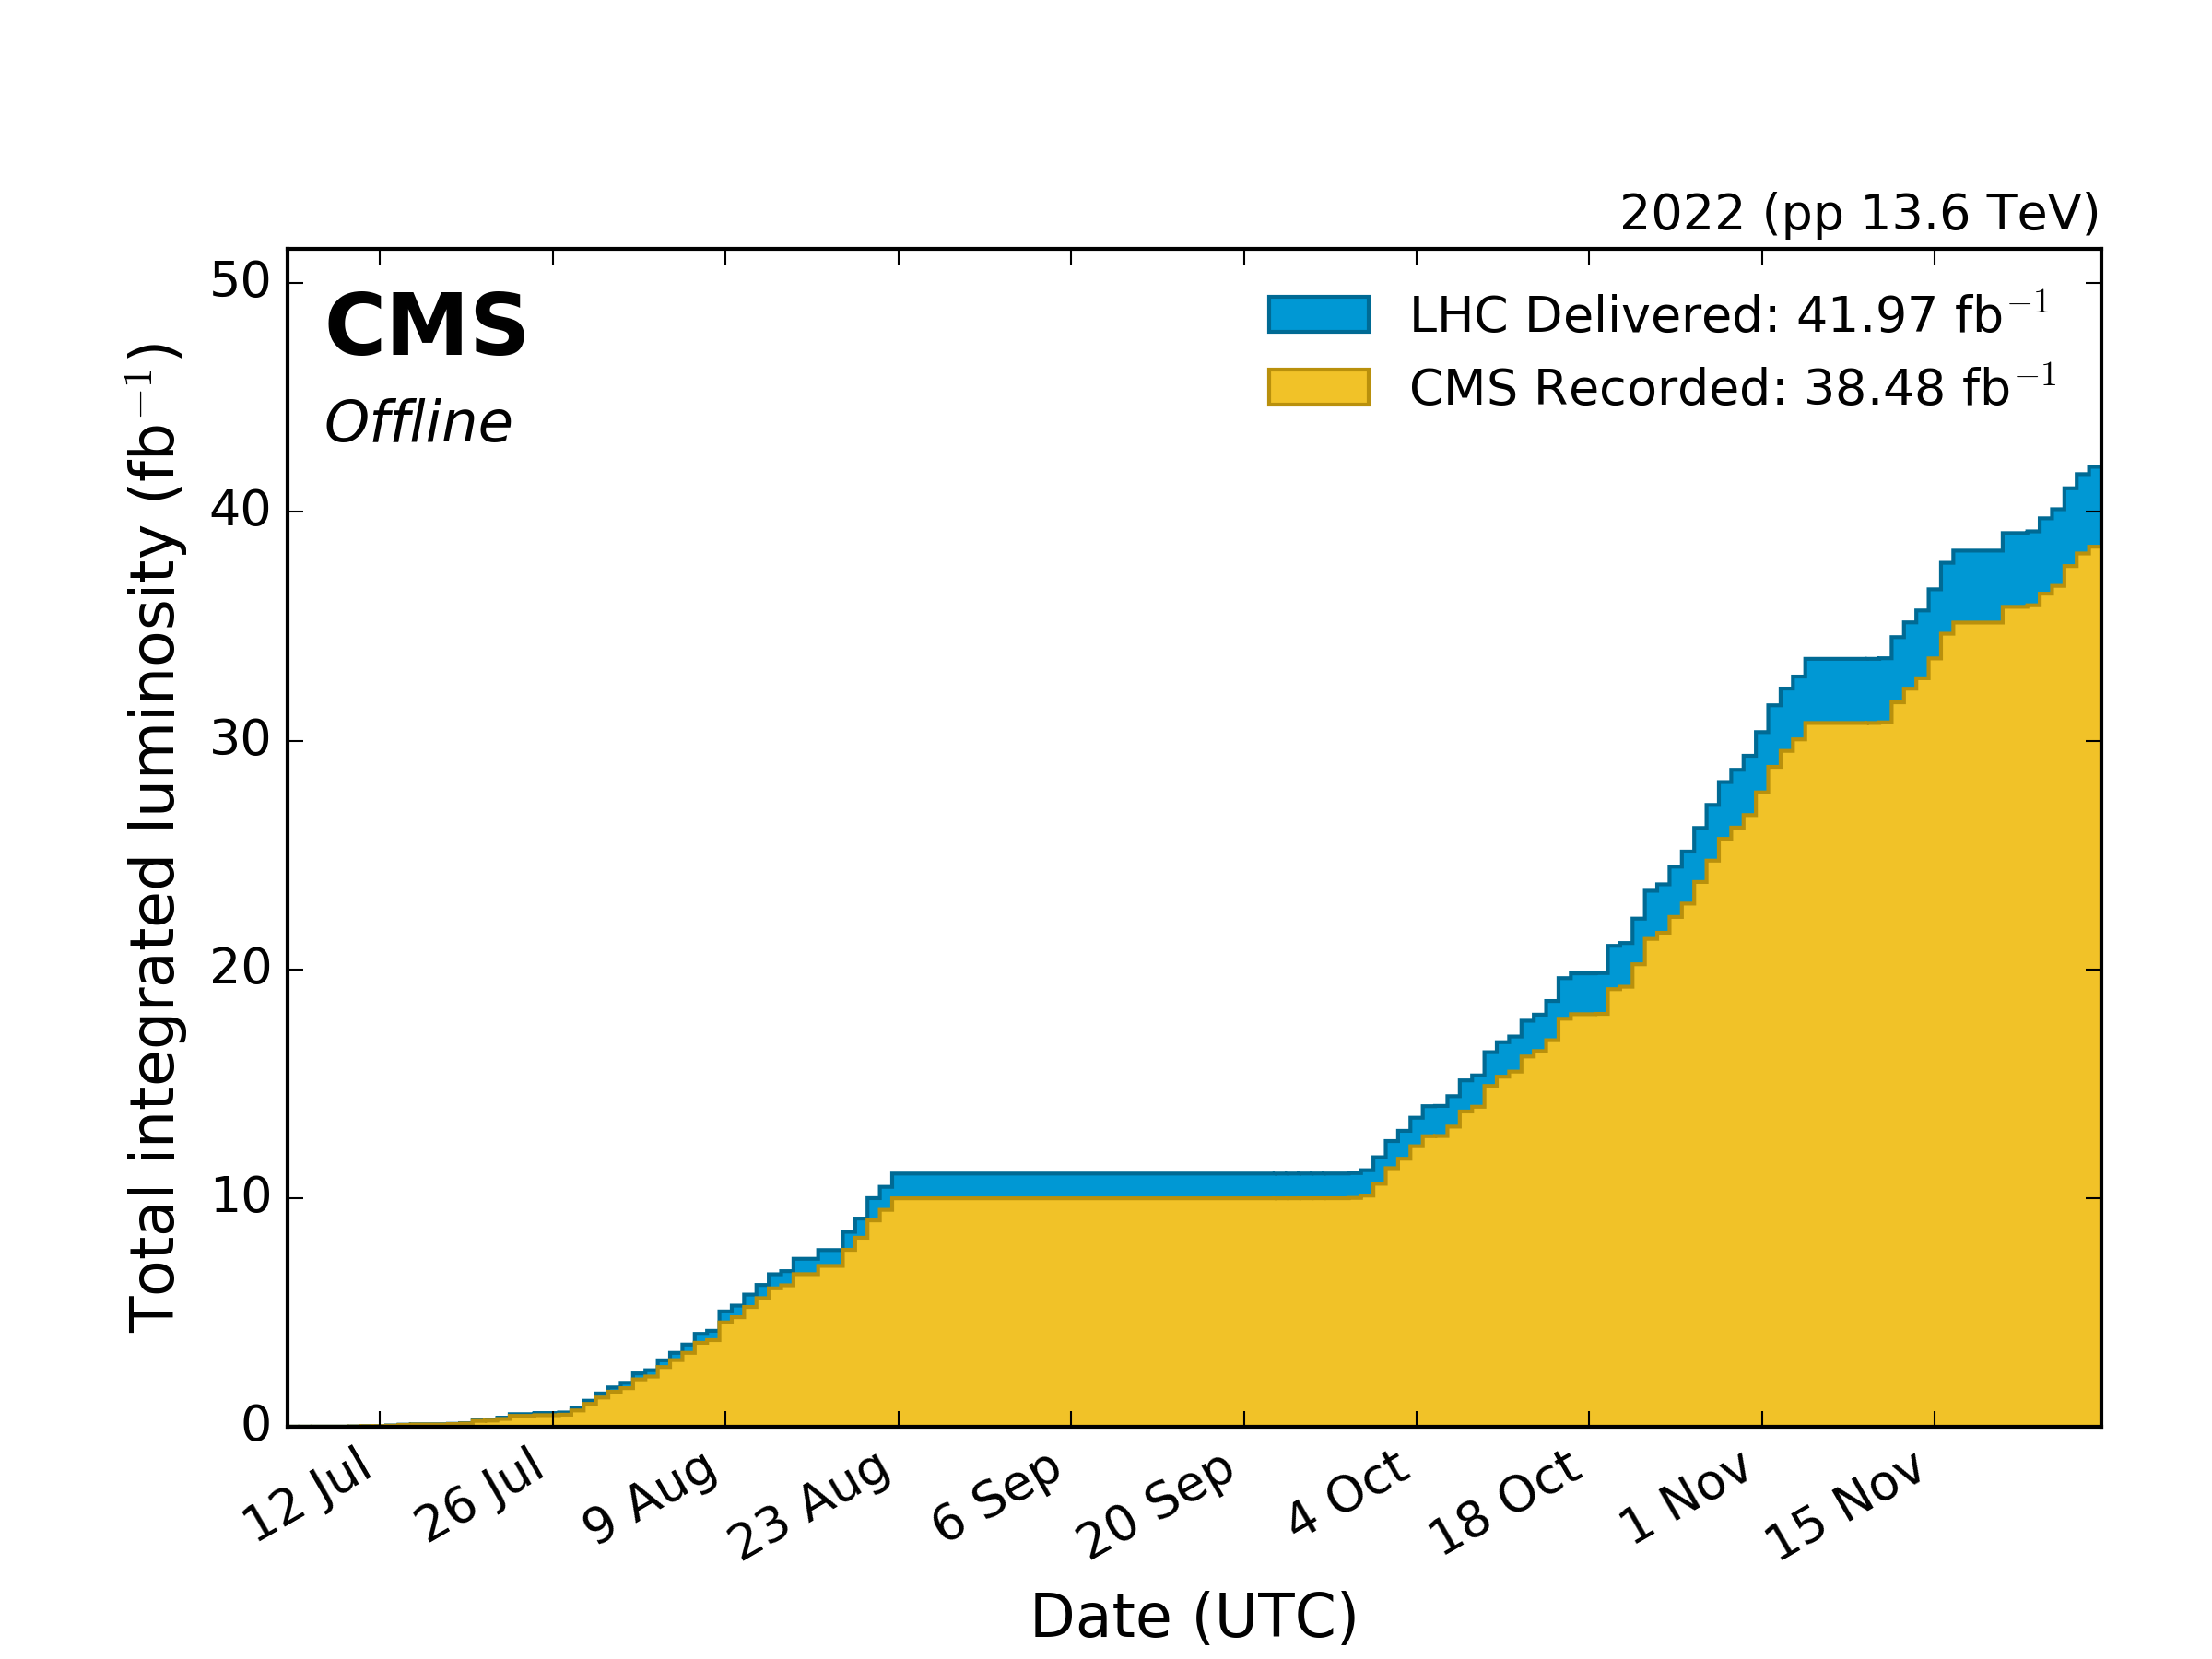
\includegraphics[width=.45\textwidth]{Chapter3/lumi_per_day_cumulative_pp_2022.png}
    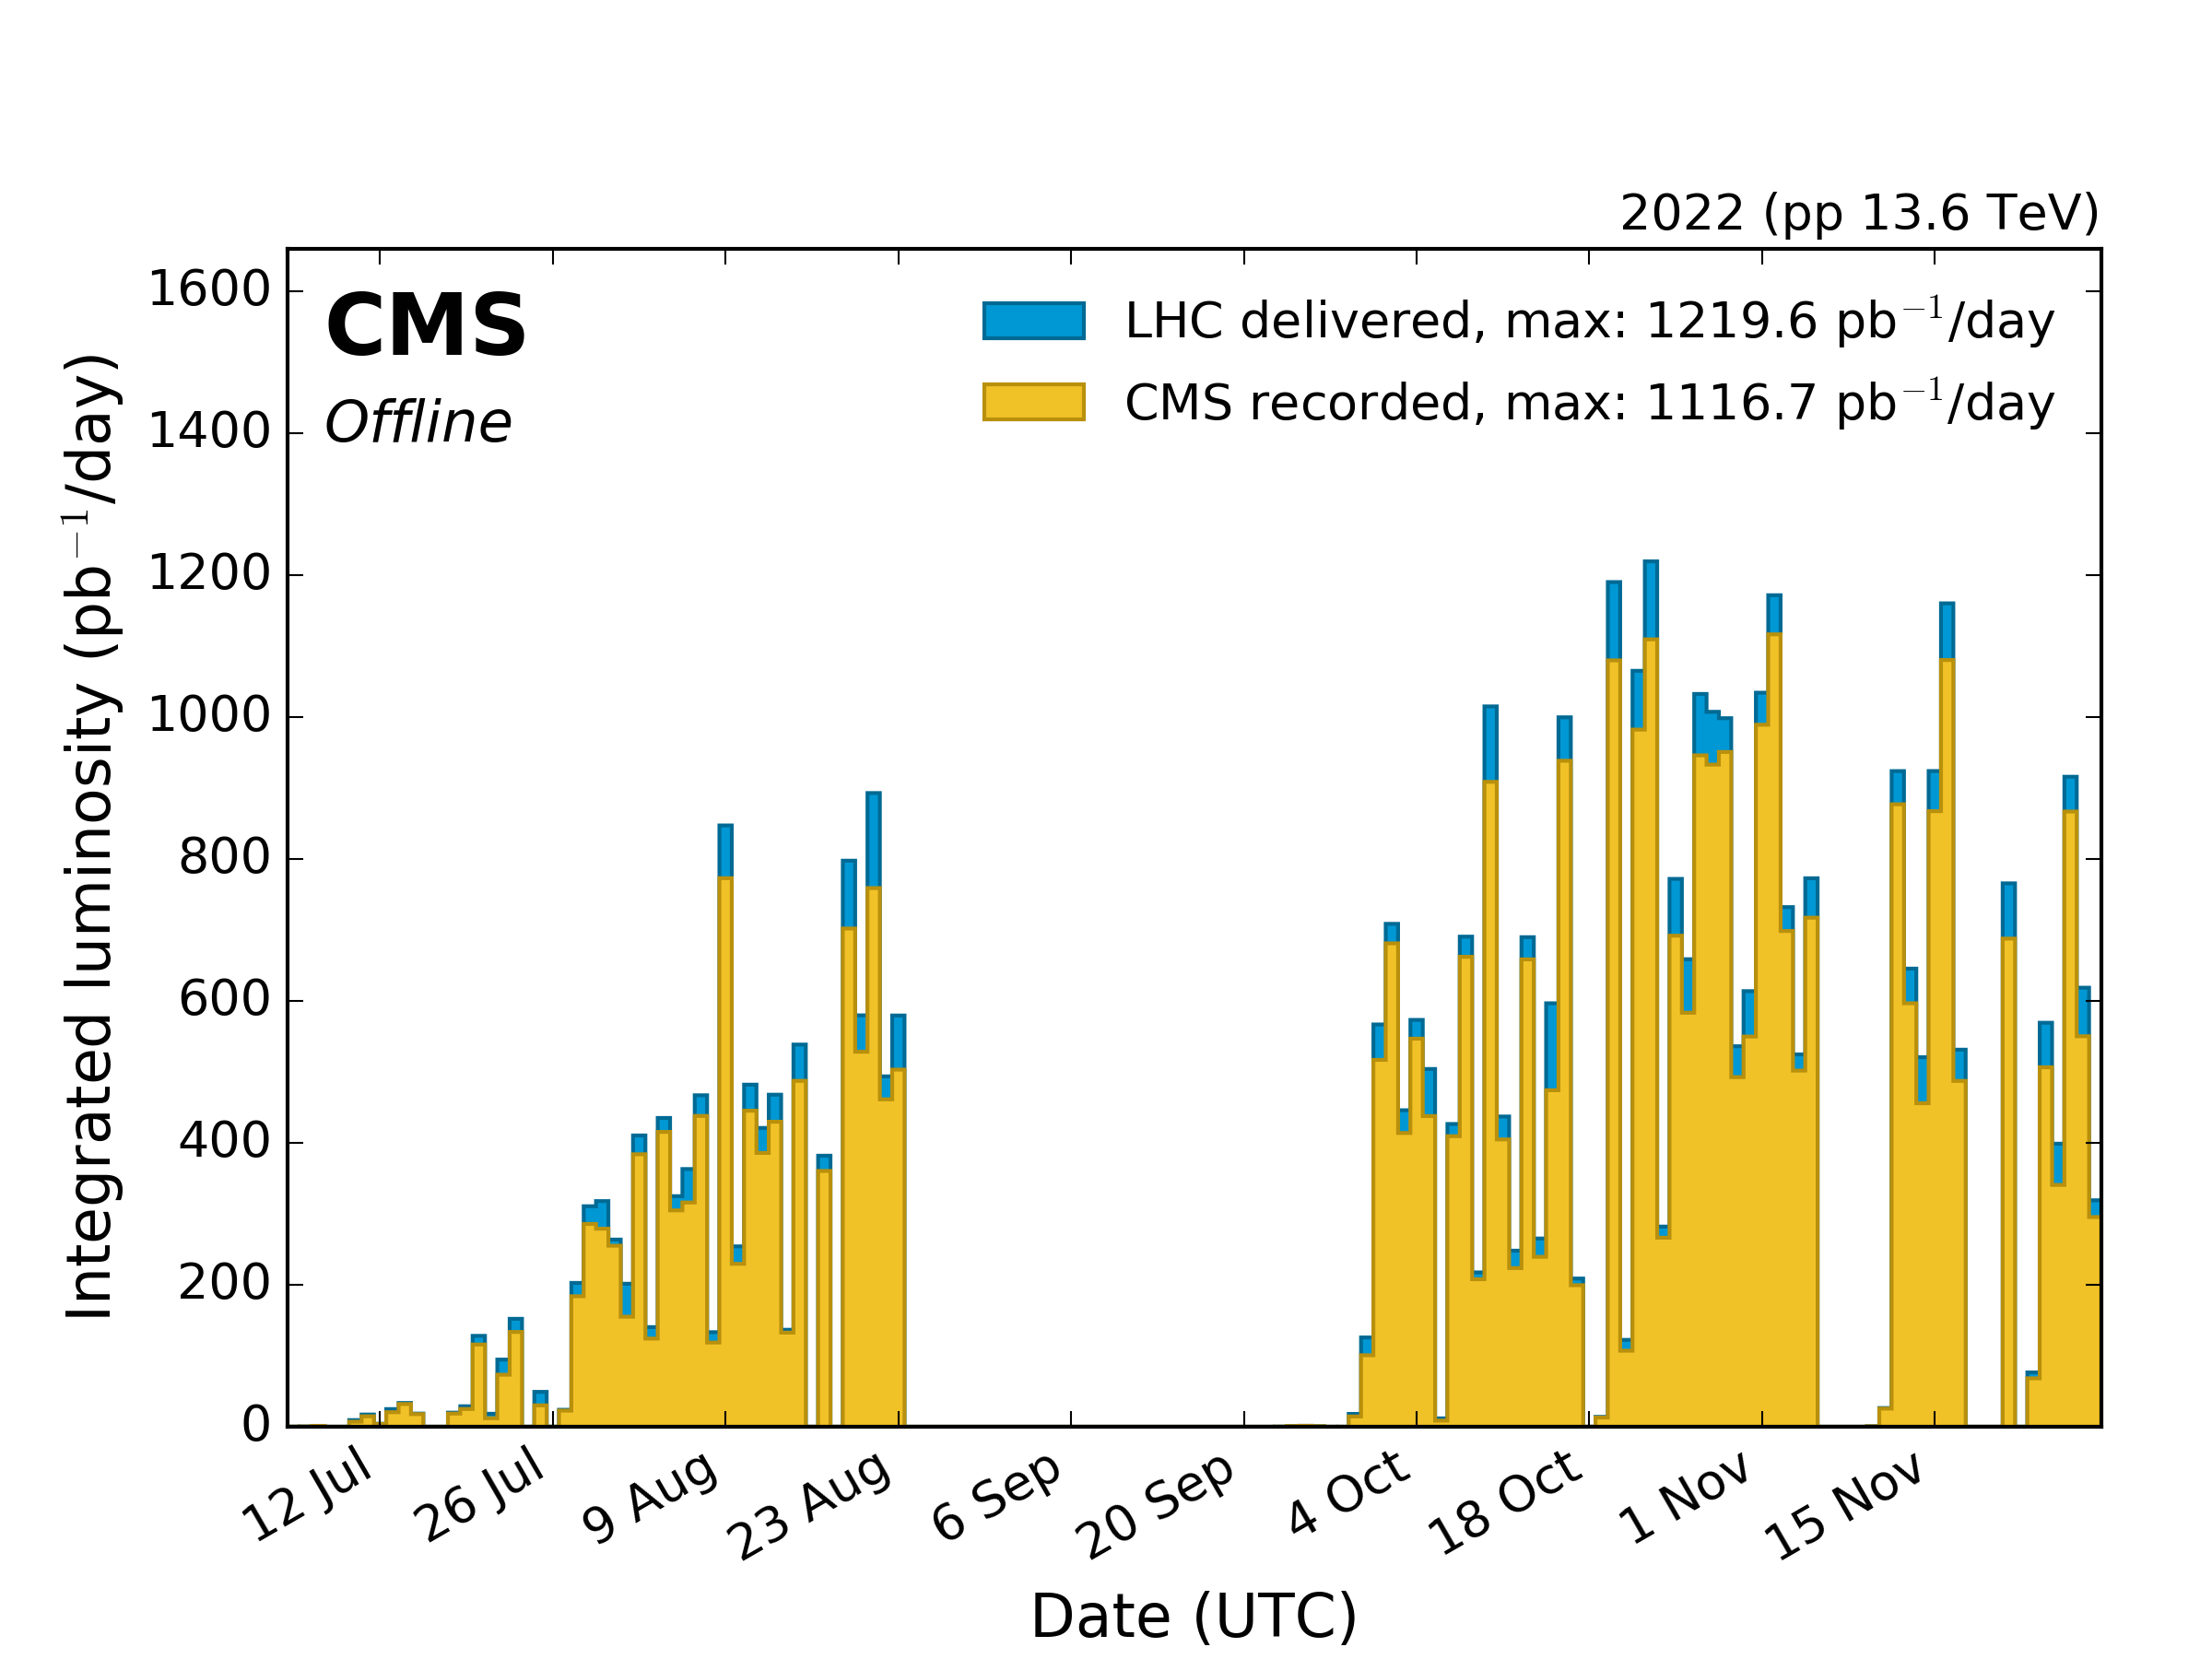
\includegraphics[width=.45\textwidth]{Chapter3/lumi_per_day_pp_2022.png}
    \caption[Integrated Luminosity 2022]{(left) Cumulative day by day integrated luminosity. (rigth) Day by day integrated luminosity, 2022 as the first plot, but not cumulative.} 
    \label{Lumi_2022}
  \end{figure}
\end{center}

\section{Module selection}

To ensure accurate luminosity measurement, a module selection is created to remove any modules exhibiting long-term performance variations, indicating a non-physical shift in their cluster counts. With a total of 1856 modules in the pixel system, all of them can be considered in the luminosity measurement; however, instabilities and non-linear effects can pose challenges for accurate measurement. Thus, to identify "good" and "stable" modules, a subset is selected by eliminating  underperforming or "bad" modules and comparing their relative contributions to the cross section. Those with relatively consistent contributions across standard physics runs are kept, while those with significant changes in their relative cross section compared to the averaged relative contribution are rejected. The Module selection is achieved  with the following procedure:

\begin{itemize}
\item Poor statistics lumisections are removed from applying selection on total PCC.
\item Barrel layer-1 modules are removed, as these modules are significantly affected by dynamic inefficiency.
\item A loose selection of 7\% based on RMS/mean frome the module weight distribution (changes in the module PCC ratio relative to the total PCC) is applied. Modules with significantly large RMS/mean are removed with this selection as shown in \ref{goodmodule}.
\item The module stability is re-evaluated based on RMS/mean values using an iterative method where the second iteration is made with a loose selection of 4\%.
\end{itemize}

\begin{center}
  \begin{figure}[h!]
    \centering
    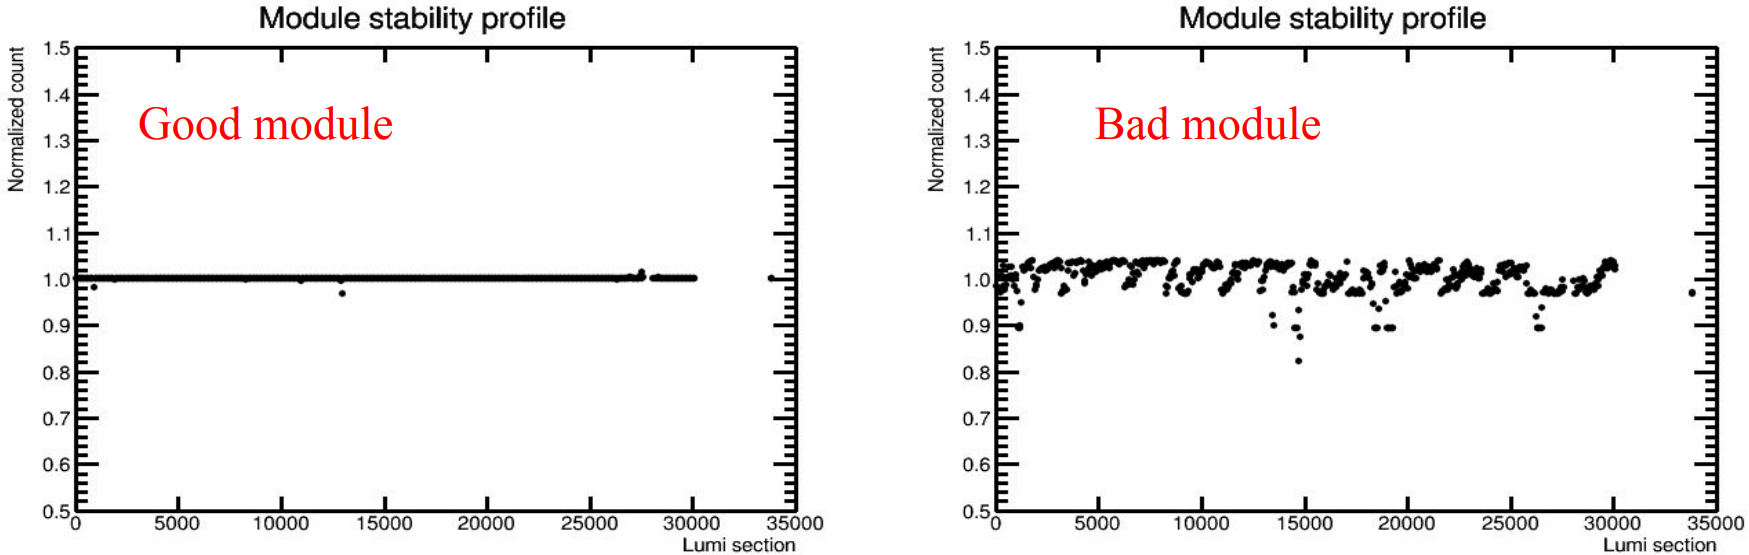
\includegraphics[scale=.17]{Chapter4/good_module.png}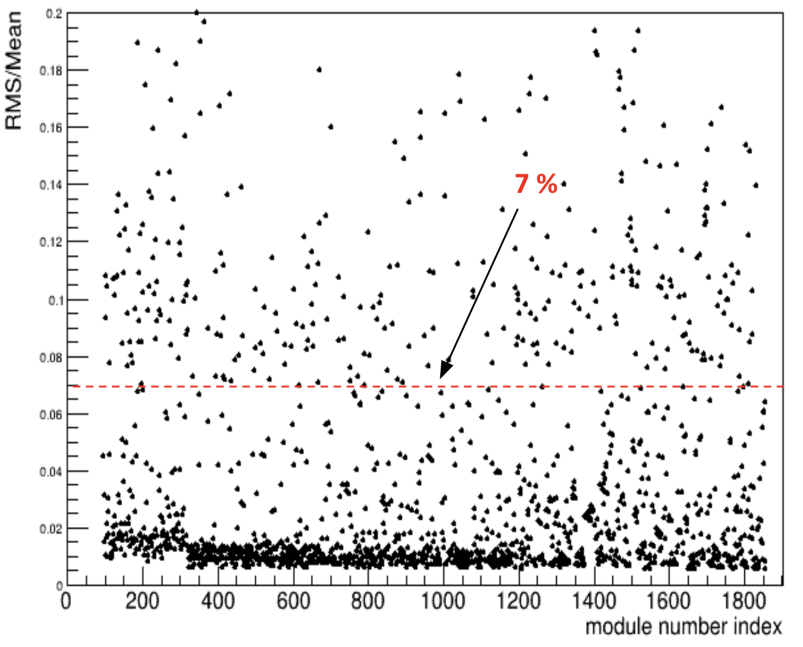
\includegraphics[scale=.15]{Chapter4/RMSmean.png}
    \caption[RMS/mean Module  Stability]{ left: stability profile for good and bad modules where weight is plotted as a function of lumi section.  Right: RMS/mean values of module weight for all pixel modules  where each pixel module is represented by a module number index (same happen for the 4\% iteration).} 
    \label{goodmodule}
  \end{figure}
\end{center}

The changing conditions of the pixel detector over time, such as detector noise, aging effects, and radiation damage, can cause variations in the number of well-performing modules during different periods. Recognizing this, these variations are evaluated over a 23-second interval, which corresponds to the granularity of the luminosity database.\\

To ensure the accuracy of the measurements, pixel module veto lists were generated for five different time periods, namely C, D, E, F, and G, using the procedure described above for each period. To further enhance the stability of the PCC measurement, a common module vetolist was created by combining the lists from all five periods were the number of bad modules per period were added and modules with equal ID were removed , as shown in table \ref{common veto module}. The PCC data with zero bias was then reprocessed using this common module vetolist and ultimately used for the vdM analysis.

\begin{table}[ht]
\centering
\caption{After each iteration for each period, the periods C and D are combined, followed by the periods C, D, and E, then the periods C, D, E, and F, and finally, the common veto list is created using the periods C, D, E, F, and G.}
\begin{tabular}{ccc}
\textbf{Period} & \textbf{\# bad modules} & \textbf{\# good modules}  \\ 
\toprule
2022C+D         & 886                     & 970                       \\
2022C+D+E       & 1106                    & 750                       \\
2022C+D+E+F     & 1307                    & 549                       \\
2022C+D+E+F+G   & 1411                    & 445                   
\label{common  veto module}   
\end{tabular}
\end{table}


\section{Luminosity calibration: van der Meer method}

As discussed in Chapter 1, the instantaneous luminosity for a single colliding bunch is described by Eq. (\ref{luminosity_2}). In practice, while the measurement of the beam currents $N_{1,2}$ is well determined, the individual proton density functions cannot be directly measured. To address this, the vdM method involves a specific machine setup that allows for the determination of the two beam overlap integrals. This is achieved by varying the separation between the beams and measuring the resulting rates, which can be used to obtain density profiles that are close to normal distributions.

\begin{equation}
\int \rho_{x1}(x) \rho_{x2}(x) dx = \frac{R_{x}(0)}{\int R_{x}(\Delta) d\Delta}
\end{equation}

where $R_{x}(\Delta)$ is the rate measured when the two beams are separated in $x$ by a distance $\Delta$; a asimilar equation can be written in $y$. Then the beam overlap width $\Sigma_{x}$ (and similarly $\Sigma_{y}$) is defined as \cite{pas_18}:

\begin{equation}
\Sigma_{x}= \frac{1}{\sqrt{2\pi}} \frac{\int R_{x}(\Delta)d\Delta}{R_{x}(0)}
\label{CapSigma}
\end{equation}

This process leads to the final expression for luminosity for a single colliding bunch:

\begin{equation}
\mathcal{L}_{inst}=\frac{N_{1} N_{2}f}{2 \pi \Sigma_{x}\Sigma_{y}}
\end{equation}

where $N_{1,2}$ are the particles per bunch (bunch current) and  $f= 11246$ Hz is the bunch orbit frequency around the LHC ring determined by the energy of the protons.\\

Therefore, the equation \ref{lumi_exp_gen} used to measure the visible cross sections $\sigma_{vis}$ takes the following form:

\begin{equation}
  \sigma_{vis}=\frac{2\pi \Sigma_{x} \Sigma_{y} R(0, 0)}{N_{1}N_{2} f}
  \label{sigmavis_eq}
\end{equation}

Experimentally, the quantities $\Sigma_{x}$ and $\Sigma_{y}$, as defined in Eq. (\ref{CapSigma}), are determined by conducting two separate scans in the $x$ and $y$ directions, respectively. 
These scans are performed by varying the separation between the beams in each direction  at a fixed number of separation steps.The separation steps are determined through curve fitting of the scan data based on the luminometer rate measurements obtained during the vdM scans.\\

The measured rate, denoted by $R(0,0)$, is determined as the highest value among the rates obtained in the $x$-scan $R_x(0)$, and the rates obtained in the $y$-scan $R_y(0)$. Although the beam widths are identical for all luminometers, the peaks of the scan curves are specific to each luminometer.\\

Figure \ref{vdm_sketch} depicts a schematic of the beam positions during vdM scans in the $x$ and $y$ planes, along with the detector rate as a function of beam separation  \cite{pas_18}.

\begin{center}
  \begin{figure}[h!]
    \centering
    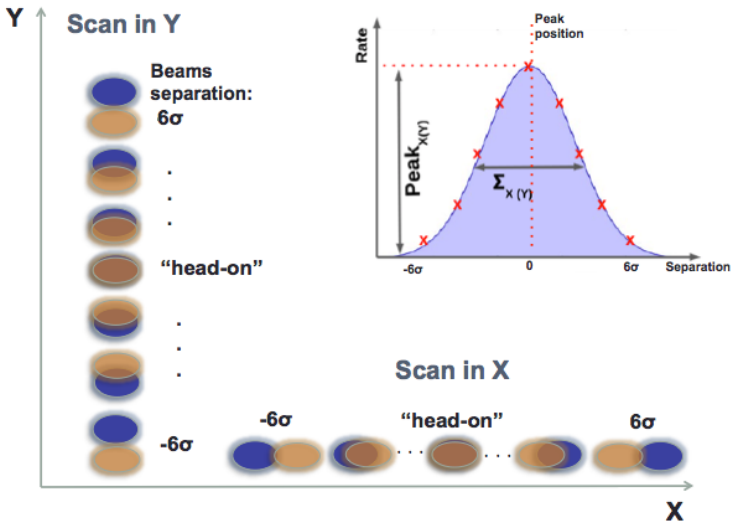
\includegraphics[scale=.37]{Chapter3/vdm_sketch.png}
    \caption[Sketch of a vdM scan in x and y planes and example of fitting resulting rates]{ The sketch of a vdM scan in $x$ and $y$ planes. The indent sketch is an example of the fit of the resulting rates \cite{vdM_sketch}.}
    \label{vdm_sketch}
  \end{figure}
\end{center}

